\section{Nature et propagation du son}
\subsection{Vitesse du son dans divers milieux}
% \begin{tabular}{lll}
% Vitesse de propagation & \(c=\sqrt{B/\rho} \) & m/s \\%\hline\rule{0pt}{15pt}\hspace{-6pt} 
% \end{tabular}
\begin{tabular}{ll|ll}
    Milieux & c (\si{\meter\per\second}) & Milieux & c (\si{\meter\per\second})\\\hline
    Air (\SI{0}{\degreeCelsius}) & 331 & Eau de mer & 1533\\
    Air (\SI{100}{\degreeCelsius} & 366 & Aluminium & 5100\\
    Hydrogène (\SI{0}{\degreeCelsius}) & 1286 & Cuivre & 3560\\
    Oxygène (\SI{0}{\degreeCelsius}) & 317 & Fer & 5130\\
    Hélium (\SI{0}{\degreeCelsius}) & 972 & Plomb & 1322\\
    Eau & 1493 & Alcool & 1143
\end{tabular}

\subsection{Fonctions d'ondes}
\begin{tabular}{lll}
% Valeur & Formule & Unité\\\hline
    Déplacement &  \(u(x,t)=A\sin (\omega t \pm kx+\phi)\) & \si{\meter}\\[5pt]
    Pression & \(p(x,t)=P_{o}\cos(\omega t \pm kx+\phi)\) & \si{\pascal}\\[5pt]
    Amplitude & \(P_{o}=\rho c \omega A\) & \si{\pascal}\\[5pt]
    Impédance & \(Z=P/V=\sqrt{B\rho}=\rho c\) & \si{\pascal\second\per\meter}\\[5pt]
    V. propagation & \(c=\sqrt{B/\rho} \) & \si{\meter\per\second}
\end{tabular}

\subsection{Intensité d'une onde}
\begin{center}
\begin{tabular}{c|c}
    Onde plane & Onde sphérique \\\hline\\[-1em]
    \(I=\frac{\rho c (\omega A)^2}{2}=\frac{P_{o}^{2}}{2\rho c}\) & \(I=\frac{W}{S}=\frac{W}{4\pi r^{2}}\)
\end{tabular}
\hspace{1em}\si{\watt\per\meter\squared}
\end{center}

% \subsubsection{Onde plane}
% \begin{center}
%     \(I=\frac{\rho c (\omega A)^2}{2}=\frac{P_{o}^{2}}{2\rho c}\) \si{\watt\per\meter\squared}    
% \end{center}

% \subsubsection{Onde sphérique}
% \begin{center}
%     \(I=\frac{W}{S}=\frac{W}{4\pi r^{2}}\) \si{\watt\per\meter\squared}    
% \end{center}

\subsection{Intensité en décibel}
\begin{center}
    \(IL=10\log\qty(\frac{I}{10^{-12}})=10\log(I)+120\) \si{\decibel}    
\end{center}

\subsection{Onde stationnaire}
% \begin{tabular}{lll}
% %Valeur & Formule & Unité\\\hline
% Déplacement & \(u(x,t)=2A\sin(kx)\cos(\omega t)\) & \si{\meter}\\
% Pression & \(P(x,t)=2P_{o}\cos(kx)\sin(\omega t)\) & \si{\pascal}
% \end{tabular}

\subsubsection{Colonne fermée aux deux extrémités (Cas général)}
\begin{tabular}{lll}
Longueur de colonne & \(L=\frac{n\lambda}{2}\) & \si{\meter}\\[8pt]
Longueur d'onde & \(\lambda_{n}=\frac{2L}{n}\) & \si{\meter}\\[8pt]
Fréquence & \(f_{n}=\frac{nc}{2L}\) & \si{\hertz}\\[8pt]
Déplacement & \(u(x,t)=2A\sin(kx)\cos(\omega t)\) & \si{\meter}\\[5pt]
Pression & \(P(x,t)=2P_{o}\cos(kx)\sin(\omega t)\) & \si{\pascal}
\end{tabular}

\subsubsection{Colonne ouverte aux deux extrémités}

\begin{tabular}{lll}
% Valeur & Formule & Unité\\\hline
% Longueur de colonne & \(L=\frac{n\lambda}{2}\) & \si{\meter}\\[8pt]
% Longueur d'onde & \(\lambda_{n}=\frac{2L}{n}\) & \si{\meter}\\[8pt]
% Fréquence & \(f_{n}=\frac{nc}{2L}\) & \si{\hertz}\\[8pt]
Déplacement & \(u(x,t)=2A\cos(kx)\sin(\omega t)\) & \si{\meter}\\[5pt]
Pression & \(P(x,t)=2P_{o}\sin(kx)\cos(\omega t)\) & \si{\pascal}
\end{tabular}

% \subsubsection{Colonne fermée aux deux extrémités}
% \begin{tabular}{lll}
% Longueur de colonne & \(L=\frac{n\lambda}{2}\) & \si{\meter}\\[8pt]
% Longueur d'onde & \(\lambda_{n}=\frac{2L}{n}\) & \si{\meter}\\[8pt]
% Fréquence & \(f_{n}=\frac{nc}{2L}\) & \si{\hertz}\\[8pt]
% Déplacement & \(u(x,t)=2A\sin(kx)\cos(\omega t)\) & \si{\meter}\\[5pt]
% Pression & \(P(x,t)=2P_{o}\cos(kx)\sin(\omega t)\) & \si{\pascal}
% \end{tabular}

\subsubsection{Colonne ouverte à une extrémité, fermée à l'autre}
\begin{tabular}{lll}
Longueur de colonne & \(L=(2n-1)\frac{\lambda}{4}\) & \si{\meter}\\
Longueur d'onde & \(\lambda_{n}=\frac{4L}{(2n-1)}\) & \si{\meter}\\[8pt]
Fréquence & \(f_{n}=\frac{(2n-1)c}{4L}\) & \si{\hertz}\\[8pt]
Déplacement & \(u(x,t)=2A\cos(kx)\sin(\omega t)\) & \si{\meter}\\[5pt]
Pression & \(P(x,t)=2P_{o}\sin(kx)\cos(\omega t)\) & \si{\pascal}
\end{tabular}

\subsection{Battement}
\begin{align*}
    P&=P_{o_{1}}\cos(\omega_1 t)+P_{{o}_{2}}\cos(\omega_2 t)\\
    P(t)&=2P_{o}\cos\qty(\frac{\omega_1-\omega_2}{2}\,t)\cos\qty(\frac{\omega_1+\omega_2}{2}\,t)
\end{align*}
\[\bar{f}=\frac{1}{2\pi}\qty(\frac{\omega_1+\omega_2}{2})=\frac{f_1+f_2}{2}\]


\subsection{Effet Doppler}
\begin{center}
    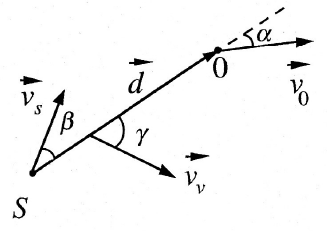
\includegraphics[width=0.25\textwidth]{fig/doppler.PNG}    
\end{center}
% \vspace{-1\baselineskip}
\[f_{o}=f_{s}\qty(\frac{c+v_{v}\cos(\gamma)-v_{o}\cos(\alpha)}{c+v_{v}\cos(\gamma)-v_{s}\cos(\beta)})\]
\begin{tabular}{ll|ll}
    Fréq. observée & \(f_{o}\) & Vitesse vent & \(v_{v}\)  \\
    Fréq. source & \(f_{s}\) & Vitesse source & \(v_{s}\) \\
    & & Vitesse observateur & \(v_{o}\)
\end{tabular}